%% USPSC-Cap2-Desenvolvimento.tex 

% ---
% Este capítulo, utilizado por diferentes exemplos do abnTeX2, ilustra o uso de
% comandos do abnTeX2 e de LaTeX.
% ---

\chapter{Methods}\label{methods}

This chapter presents the workflow and methodology underlying the use of the Yara robotic system for SEEG surgery. It begins with patient monitoring and data acquisition (Sec. \ref{sec:monitoring}), then describes the planning phase, including image fusion and electrode placement (Sec. \ref{sec:planning}). The subsequent robot-scan registration phase (Sec. \ref{sec:registration}) addresses the alignment of preoperative imaging with the robotic system. The intraoperative phase (Sec. \ref{sec:operation}) outlines the integration of robotic assistance for electrode insertion. The chapter concludes with the methods and results of system accuracy evaluation and validation (Sec. \ref{method-results}).

\section{Patient Monitoring}\label{sec:monitoring}

Patient monitoring for SEEG candidates involves comprehensive video-EEG and MRI assessments to localize epileptogenic zones and determine surgical eligibility, as detailed in Sec. \ref{sec:non-invasive-eeg}. Once a focal epilepsy amenable to surgical intervention is identified, and SEEG is selected as the preferred invasive technique, the workflow proceeds to the planning phase, where the robotic system assists in precise electrode trajectory definition.

\section{SEEG Planning Phase}\label{sec:planning}

The user interface is prepared for SEEG planning, developed to address neurosurgeons' and neurologists' needs during planning. The goal of planning is to select target points so that the electrodes cross the most probable epileptogenic zone. Entry points need to be selected so that the electrode trajectory is safe and follows a path without collision with critical structures such as arteries or eloquent regions of the brain. Typically, electrodes have between 5 and 15 contacts along their length, spaced by a couple of millimeters. Between 5 and 10 electrodes are placed in the SEEG procedure.

For SEEG planning, the surgeon requires MRI images to visualize soft tissues, brain structures, and vascularization, as well as CT images that provide precise information about the skull. Combining these modalities through image fusion enables the simultaneous assessment of critical anatomical features, such as blood vessels, gray and white matter, and bone structures in a unified reference frame. This alignment is essential for safe and effective electrode placement, as it allows the surgeon to avoid critical regions and optimize the trajectory of each electrode.

\subsection{Image Fusion}

For image fusion, we adopted the method described in \cite{klein2009evaluation}, which enables the alignment of CT-CT, MRI-MRI, or CT-MRI images. The fusion process aims to optimize the mutual information metric, identifying the transformation that best aligns a source image with a target image. In multimodal fusion scenarios such as CT-MRI, the images differ in tissue representation and contrast (bone appears bright in CT but is nearly invisible in MRI). Mutual information serves as a statistical measure of the shared information between two random variables. In image registration, it quantifies how well one image explains the other, independent of intensity values, making it effective for multimodal image alignment.

% TODO
% Figure \ref{} shows an example of CT-MRI image fusion for a 9-years old patient.

\subsection{Electrode Placement}

After analyzing the images, electrodes can be planned by determining the entry and target points, the type of electrode containing basic information such as spacing, coordinates, number of contacts, and the dimensions of each electrode. This step is performed a couple of days before the surgery; the planned electrode is saved and loaded on the day of the surgery into the interface. Small adjustments can be made during the surgery if needed.

\section{Robot-Scan Registration Phase}\label{sec:registration}

Before starting the operation, it is essential to perform a registration procedure to align the coordinate systems of the preoperative scans and the robot. This step ensures that the positions of the planned electrode trajectories correspond accurately to the physical space in which the robot operates. The registration method adopted in this work is known as fiducial registration, which involves identifying and matching a set of anatomical or artificial landmarks (fiducials) in both the image space and the physical space. By determining the transformation that best aligns these corresponding fiducial points, the system can accurately map planned positions from the imaging data to the robot's coordinate system \cite{zeng2017surgical}. This alignment is fundamental for transferring surgical plans to the robotic system and ensuring precise execution during the procedure.

The procedure begins by identifying several fixed anatomical or artificial landmarks, known as fiducial points, within the preoperative images. These same points are then physically located on the patient using the robotic arm. To record each corresponding point, the operator positions the robot's tool at the desired location and confirms the selection. The collected coordinates are transmitted to the robot's control module, which computes the optimal rigid transformation using the ICP method.

% TODO, it's not the ICP, it's the Umeyama
Expanding on the ICP method by \cite{slambook}, the goal is to find the matrix \textbf{R} and vector \textbf{t} that best solve the Euclidean transformation \ref{eq:icp} given a matched set of 3D points like $\textbf{P}=\{\textbf{p1}, ... , \textbf{p}_n\}$ and $\textbf{P'}=\{\textbf{p'1}, ... , \textbf{p'}_n\}$.

\begin{equation}
    \forall i, \textbf{p}_i = \textbf{Rp'}_i+ \textbf{t} 
    \label{eq:icp}
\end{equation}

In this procedure, fiducial landmarks are selected that are anatomically distinct and reproducible points on the patient's head, reliably identifiable both in the CT/MR images and in physical space. Commonly used fiducials include the nasion (the indentation between the forehead and the nose), the left and right preauricular points (just in front of each ear), and sometimes additional points such as the tip of the nose or the outer canthi. These landmarks are chosen for their ease of identification and for exhibiting minimal movement relative to the skull, avoiding soft‑tissue deformation.

The system computes the transformation ${}^{robot}T_{scan}$ that best aligns the two sets of points, minimizing the reprojection error and ensuring that the planned trajectories in the image space correspond precisely to the patient's anatomy in the real world. The reprojection error is computed by transforming the fiducial points in the scan space ($^{scan}P_{virtual}$) to the robot space and comparing with the collected fiducials ($^{robot}P_{real}$) in the target space (Equation \ref{eq:reproj}).

\begin{align} \label{eq:reproj}
Reproj = || {}^{robot}P_{real} - {}^{robot}T_{scan} \; {}^{scan}P_{virtual} ||
\end{align}


\section{Intra-Operation Phase}\label{sec:operation}

The next step is the surgery for the precise placement of electrodes in the patient. The system incorporates a digital twin of the robot within its interface, providing real-time visualization of the robot’s position and planned movements. Before executing any planned motion, the system displays the intended trajectory and requires explicit confirmation from the operator. This workflow ensures that each step of the surgical process is performed with maximum safety and situational awareness.

During the trepanation process, the system assists the surgeon by displaying the precise drilling depth required to safely penetrate the skull without breaching the dura-mater. Once the bone has been traversed, a drill guide is positioned to maintain the correct trajectory and stabilize the electrode. The interface then provides the exact insertion depth needed for the electrode to reach the planned intracerebral target, ensuring accurate and safe placement.

% \chapter[Experiments Setup]{Experiments Setup}
% \label{experiments-setup}

\chapter[Method and Results]{Experiments and Results}
\label{method-results}

As discussed in Sec. \ref{sec:seeg-methods}, an SEEG method must be sufficiently accurate to place each electrode at the planned position and orientation. The accuracy can be measured by 
the Euclidean distance between the planned entry point and the entry point achieved after the surgery. The same method applies to the target point. The angle between the entry-to-target vector $\vec{P_{target}} - \vec{P_{entry}}$ for the planned electrodes and the post-surgery electrodes reflects the orientation error. 

To comprehensively assess the accuracy of Yara system for SEEG surgeries, we developed and tested three distinct phantom models, each with a dedicated evaluation setup: (1) a conical target phantom in a mock-OR, (2) a synthetic brain phantom in a mock-OR, and (3) a synthetic brain model assessed under actual OR conditions.

The experiments were conducted in a controlled laboratory environment designed to closely mimic the conditions of an actual operating room. This setup included a surgical table, a head clamp for securing the phantom or synthetic head, and the complete robotic system mounted on its dedicated cart. The laboratory environment allowed for iterative testing and refinement of the workflow, ensuring that all components of the system functioned as intended before transitioning to a clinical setting.

Following laboratory assessments, the system was evaluated in OR at the Hospital das Clínicas da Faculdade de Medicina de Ribeirão Preto (HC-FMRP-USP). In this environment, the robot and its cart were transported and installed according to standard OR protocols. The tests in the OR aimed to assess the system's performance under actual clinical conditions, including the presence of medical staff, and integration with existing surgical infrastructure.

\section{Conical Target Phantom}

To validate the system's accuracy using a phantom, we employed a 3D-printed phantom of a child's head along with a base containing cylinders topped with cones (the patient data used for the phantom model was approved for research use, and no personal or identifiable information is available). The apex of each cone served as a target point, requiring the system to position a thin metal rod - simulating an electrode - precisely at these locations. During the planning phase, entry points were arbitrarily distributed across the skull surface to maximize variability, while target points corresponded to the cone peaks. Registration was performed using fiducial markers placed on the head surface, following the same protocol as the synthetic brain validation.

\begin{figure}
    \centering
    \includegraphics[width=0.95\textwidth]{USPSC-img/conical-targets-phantom.png}
    \caption{Conical targets phantom used for quantitative accuracy assessment via stereoscopic imaging.}
    \label{fig:conical-phantom}
\end{figure}

During the operation phase, the robot sequentially positioned itself at each planned electrode site. The interface provided the required drilling depth, guiding the placement of the drill stop, and calculated the insertion length needed for the rod to reach the target point.

To measure the accuracy of the system, we utilized a stereo camera setup to capture images of the phantom after rod insertion. The stereo camera allowed for precise measurement of the distance between the tip of the inserted rod and the apex of each cone, representing the planned target point.

\begin{figure}[h]
    \centering
    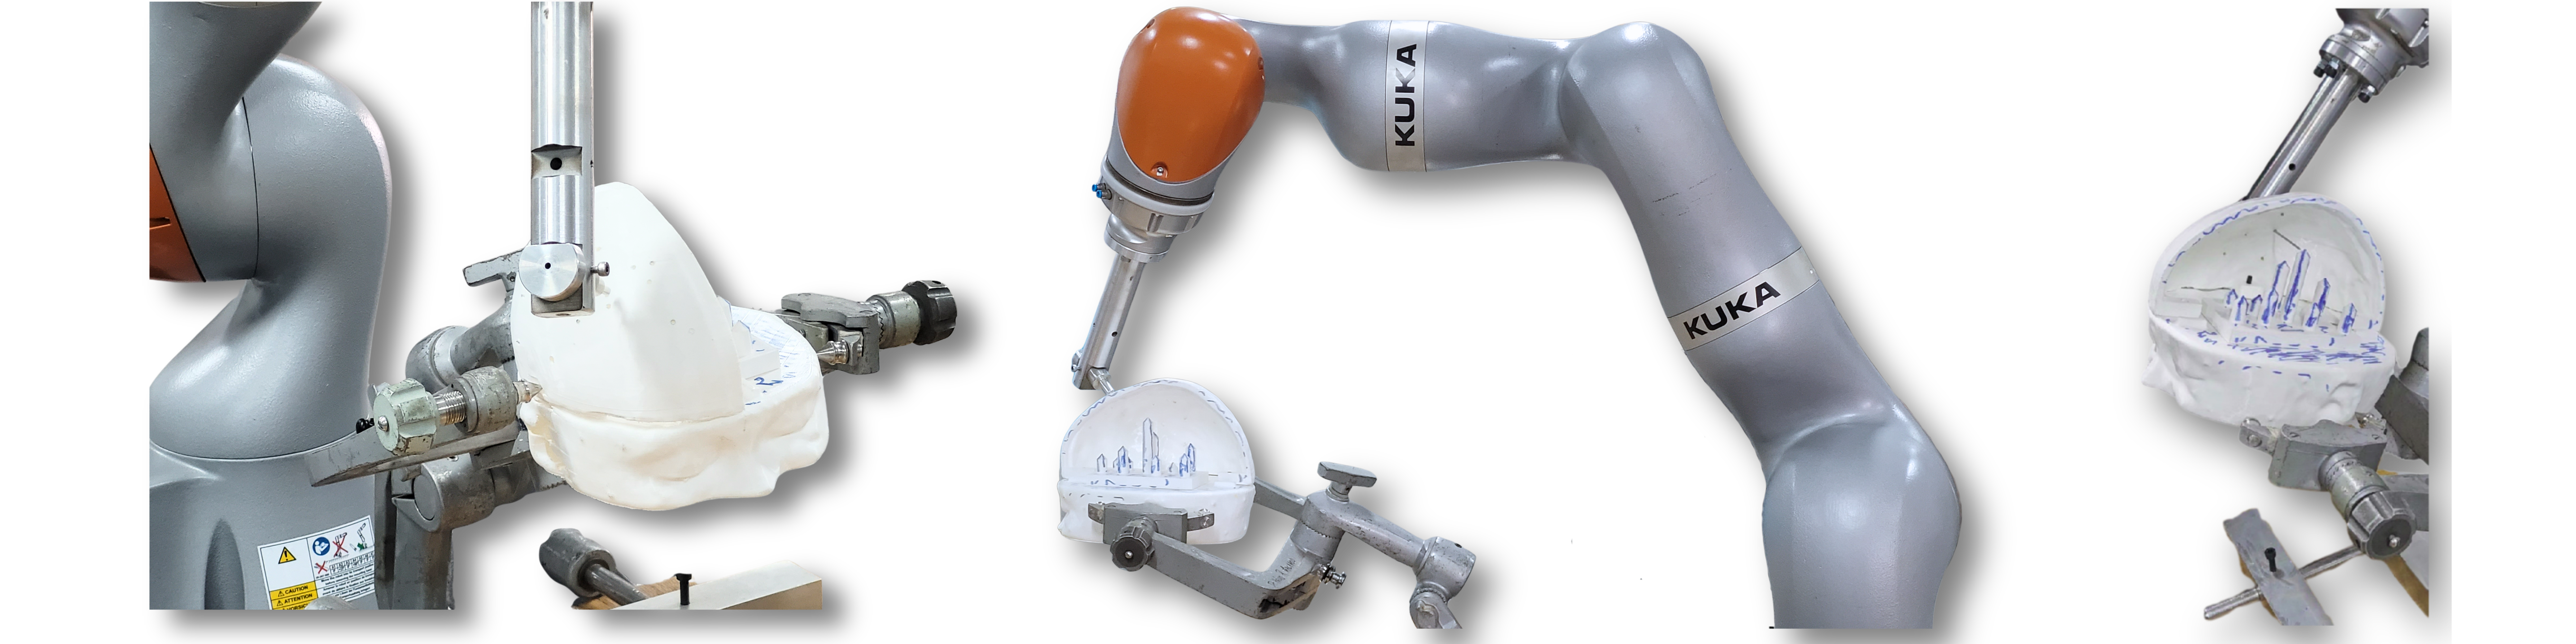
\includegraphics[width=0.99\textwidth]{USPSC-img/conical-targets-phantom-se-robot.png}
    \caption{Conical targets phantom in SE for metal rods positioning using the robotic system.}
    \label{fig:phantom}
\end{figure}

The stereo image pair was acquired using a rectified stereo camera with a 4~cm baseline and a resolution of 1920$\times$1080 pixels, with known intrinsic parameters. The tip of the rod and the cone apex were manually marked in both images, with an average marking error of proportional to the depth. We assumed a linear disparity pixel error (the error of a point in the left image and its corresponding point in the right image) of 0 to 5 pixels from 0 to 2.5 meters. The depth error was calculated using the Formula \ref{eq:depth-error}, where $z$ is the depth, $e_{\text{disp}}$ is the disparity error in pixels, $b$ is the distance between the cameras in meters, and $f$ is the focal length in pixels. The demonstration of Eq. \ref{eq:depth-error} is shown in Eq. \ref{eq:depth-error-demo}.

\begin{equation} \label{eq:depth-error}
    \delta z = \frac{z^2 e_{\text{disp}}}{f b + e_{\text{disp}}z}
\end{equation}

\begin{equation} \label{eq:depth-error-demo}
    z = \frac{f b}{d} \Rightarrow \delta z = z - z' = \frac{f b}{d} - \frac{f b}{d + e_{\text{disp}}} = \frac{f b e_{\text{disp}}}{d(d + e_{\text{disp}})} = \frac{z^2 e_{\text{disp}}}{f b + e_{\text{disp}}z}
\end{equation}

\begin{figure}[h]
    \centering
    \includegraphics[width=0.8\textwidth]{USPSC-img/phantom-rs-sample.png}
    \caption{Examples of stereo camera images used to measure the distance between the metal rod tip and the planned target point. The top and bottom rows show the left and right images of a stereo pair for the same moment in time.}
    \label{fig:phantom-rs}
\end{figure}

Using the Eq. \ref{eq:depth-error}, it was possible to estimate a maximum measurement error of 0.3~mm, which corresponds to the largest expected uncertainty in the distance calculation due to stereo camera disparity error. Nine electrodes were inserted, followed by the target error estimation process. Fig. \ref{fig:phantom} presents the phantom and Fig. \ref{fig:phantom-rs} presents images from the stereo camera used to calculate the error. Table \ref{tab:phantom-errors} presents the target error for each electrode, resulting in an average error of $1.8 \pm 0.3$ mm.

\begin{table}
    \centering
    \begin{tabular}{|c|ccccccccc|c|}
    \textbf{Electrode} & \textbf{1} & \textbf{2} & \textbf{3} & \textbf{4} & \textbf{5} & \textbf{6} & \textbf{7} & \textbf{8} & \textbf{9} & \textbf{Mean} \\
     $\Delta$ Target (mm) & 1.5 & 1.3 & 2.7 & 1.6 & 2.5 & 2.3 & 1.1 & 1.9 & 1.4 & $1.8 \pm 0.3$ \\
        \end{tabular}
    \caption{Error in the positioning of target points planned and reached after surgery using a model with phantom and stereo camera to measure distances.}
    \label{tab:phantom-errors}
\end{table}

\section{Synthetic Brain Phantom}

\begin{figure}[ht]
    \centering
    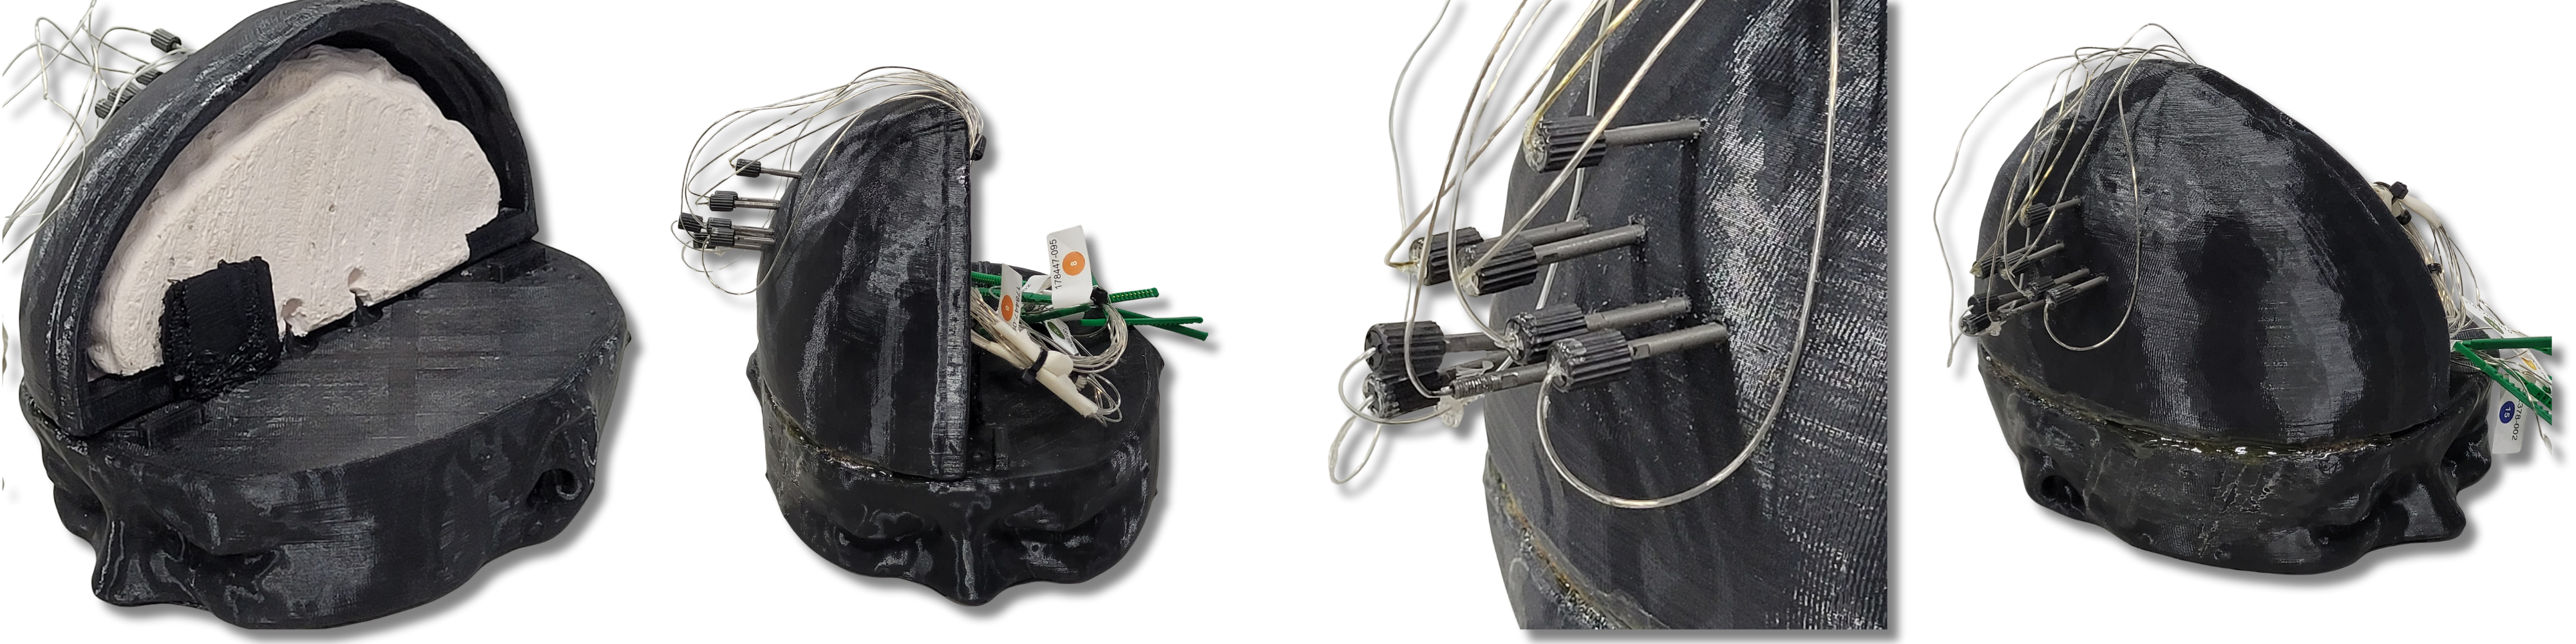
\includegraphics[width=0.95\textwidth]{USPSC-img/synthetic-brain-phantom.png}
    \caption{Phantom model with synthetic brain produced using silicone rubber and 3D printed plastic surface skin after electrode placement.}
    \label{fig:synthetic}
\end{figure}

To further evaluate the system, tests were conducted using a synthetic brain phantom. The phantom was created by molding the right hemisphere of the brain from silicone rubber to closely mimic the anatomical structure and consistency of real brain tissue. A 3D-printed head model was used to replicate the patient's head surface, including a section of the skull. This setup allowed for a realistic simulation of the SEEG procedure, enabling the robotic system to perform electrode placement in a controlled environment.

\begin{figure}[ht]
    \centering
    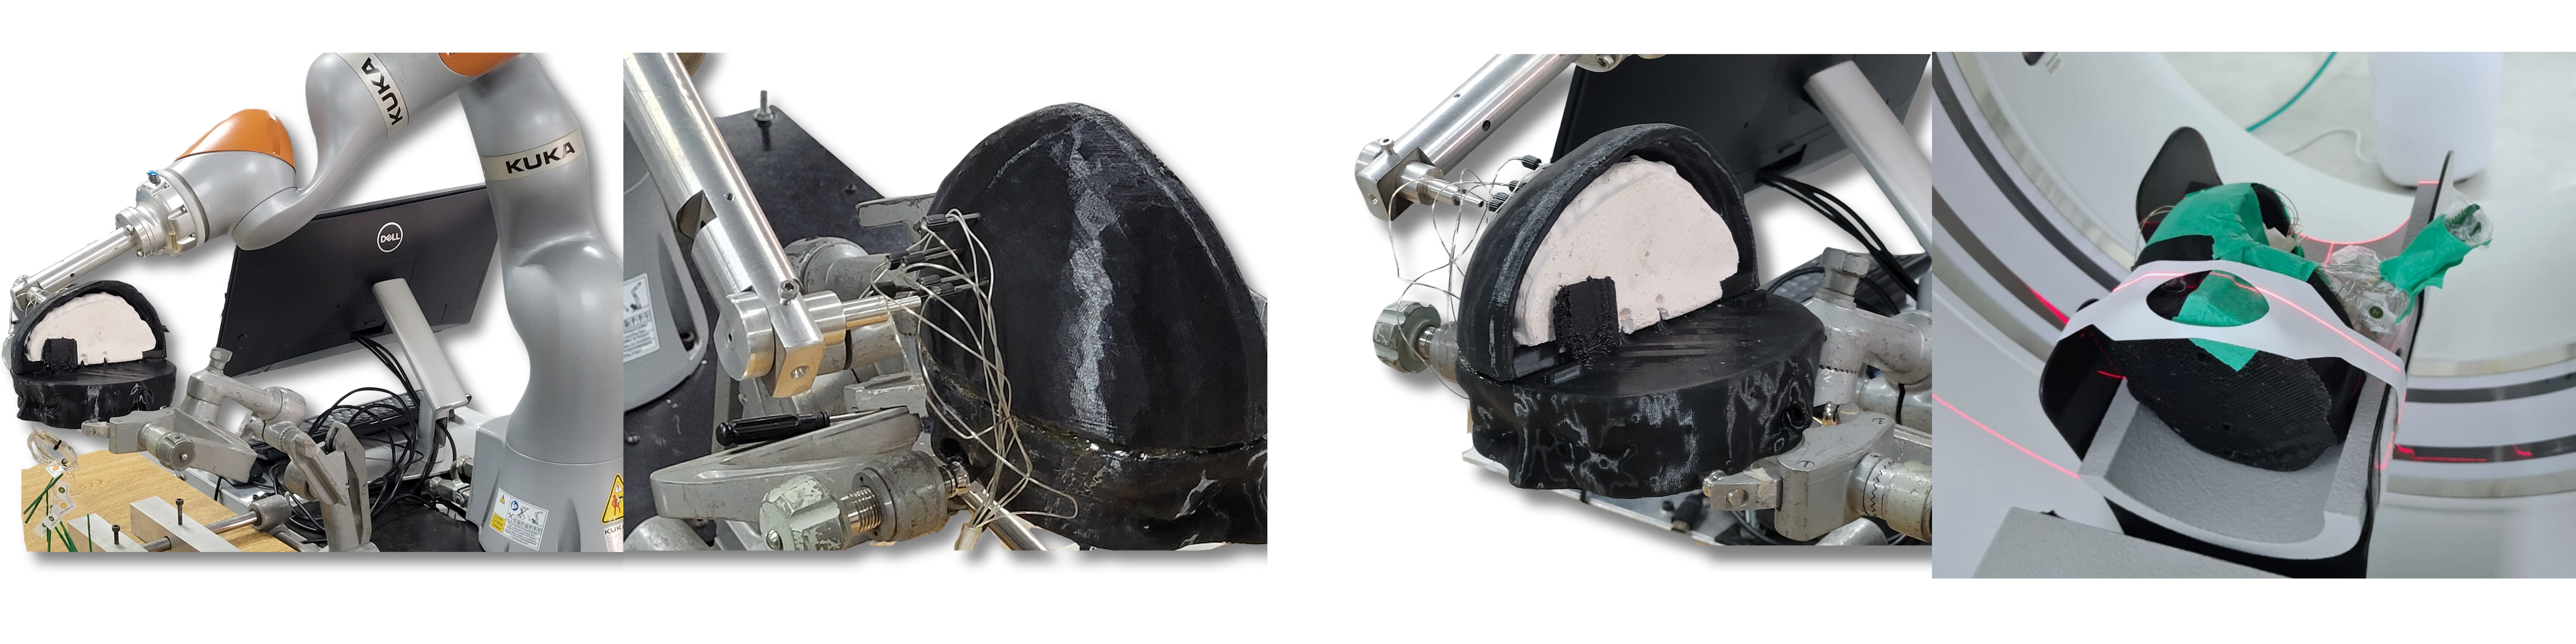
\includegraphics[width=0.95\textwidth]{USPSC-img/synthetic-brain-phantom-se-robot.png}
    \caption{Synthetic brain phantom in mock-OR during electrode placement with the robotic system. The rightmost image displays the postoperative CT scan of inserted electrodes.}
    \label{fig:sintetic}
\end{figure}

A 3D-printed positive model of the brain was produced from patient imaging data. This positive was used to create a negative mold using silicone rubber. Once cured, the negative mold was filled with silicone rubber of Shore A 5 hardness, chosen to approximate the mechanical properties of brain tissue. To facilitate demolding, a release agent was applied to the mold surface. The resulting synthetic brain was then positioned inside the 3D-printed head model, which incorporated a section of the skull to closely replicate the patient anatomy (Figure \ref{fig:synthetic}).

Preoperative CT scan and a surgical plan were used to replicate the clinical scenario in a controlled laboratory environment. The robotic system was then employed to insert nine electrodes according to the planned trajectories. The procedure was completed successfully, demonstrating the system's ability to perform electrode placement in a surgical simulation.

After the operation, the phantom with the electrodes placed invasively was taken for tomography to acquire images that show the internal positioning of the electrodes. Through this, it was possible to compare the positioning of the inserted electrodes with the surgical planning and the desired trajectories for each electrode, seeking to calculate the system error. As presented in Section \ref{sec:methods}, the error between the planned entry and target points and those achieved postoperatively are evaluation metrics for SEEG surgery and were calculated in this process.

Figure \ref{fig:synthetic} shows the synthetic model developed. The comparison between the planned and achieved electrodes with the fusion of the postoperative CT with the preoperative images (Fig. \ref{fig:sintetic-ct}) allows the calculation of Euclidean distances between the planned and achieved trajectories and, therefore, allows the evaluation of the system's accuracy (Table \ref{tab:synthetic-errors}). The CT volume has a slice spacing of 0.25 mm on the three dimensions between slices, used as the measurement error.

\begin{figure}
    \centering
    \includegraphics[width=0.95\textwidth]{USPSC-img/sintetic-brain-ct.png}
    \caption{Comparison between preoperative (red and green lines) and postoperative (gray contacts) electrode trajectories using CT scan of the synthetic brain model in the mock-OR.}
    \label{fig:sintetic-ct}
\end{figure}


 \begin{table}
 \centering
 \begin{tabular}{|c|cccccc|cc|}
 \textbf{Electrode} & \textbf{1} & \textbf{2} & \textbf{3} & \textbf{4} & \textbf{5} & \textbf{6} & \textbf{7} & \textbf{Mean} \\
 $\Delta$Entry (mm) & 1.47 & 1.81 & 1.58 & 1.71 & 0.56 & 0.95 & 1.04 & $1.30 \pm 0.25$ \\
 $\Delta$Target(mm) & 2.57 & 2.62 & 3.72 & 2.26 & 4.88 & 3.48 & 1.97 & $3.07 \pm 0.25$ \\
 \end{tabular}
 \caption{Error in positioning the entry and target points planned and reached after surgery using a synthetic brain model.}
 \label{tab:synthetic-errors}
 \end{table}

\begin{figure}[ht]
    \centering
    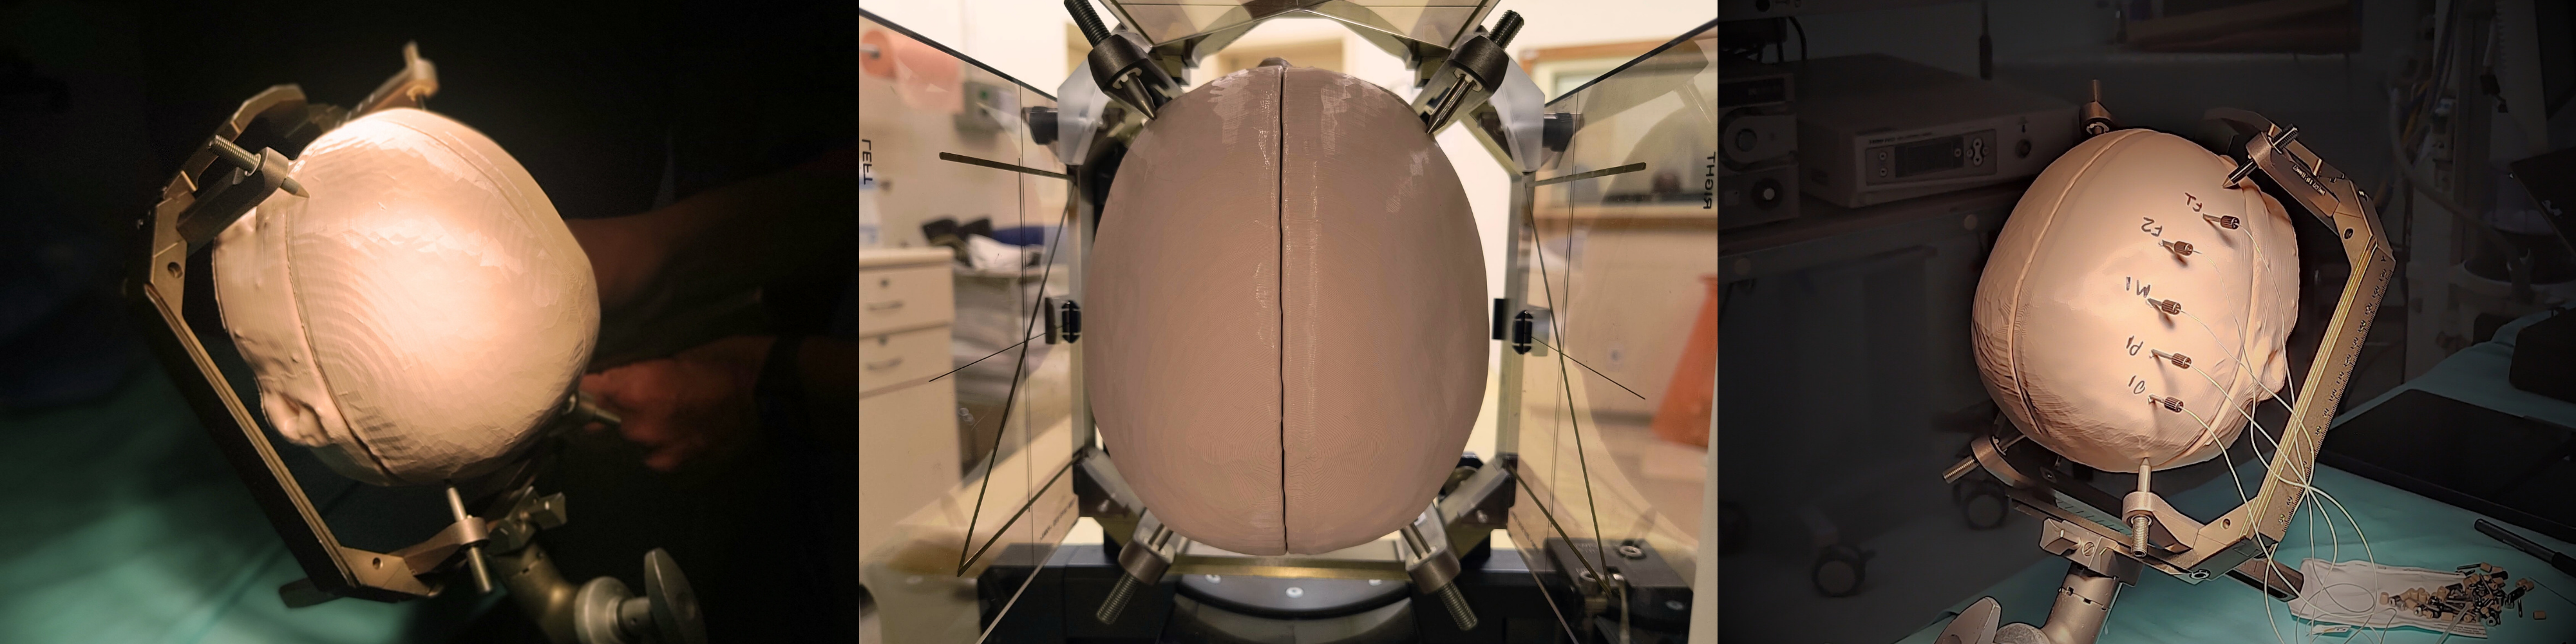
\includegraphics[width=0.95\textwidth]{USPSC-img/synthetic-brain-phantom-or-leksell.png}
    \caption{Phantom model with synthetic brain placed in the OR using stereotactic frame for electrode placement.}
    \label{fig:synthetic-or-leksell}
\end{figure}

Some limitations were observed during the tests, particularly regarding the adhesion between the electrodes and the silicone rubber material. This adhesion increased friction and made electrode insertion more difficult compared to real brain tissue, where such resistance is not typically encountered. As a result, the insertion process in the phantom did not fully replicate the ease of electrode placement observed in clinical practice. Nevertheless, the synthetic brain phantom provided a valuable platform for simulating electrode placement and quantitatively assessing system accuracy under controlled conditions.


\begin{figure}[ht]
    \centering
    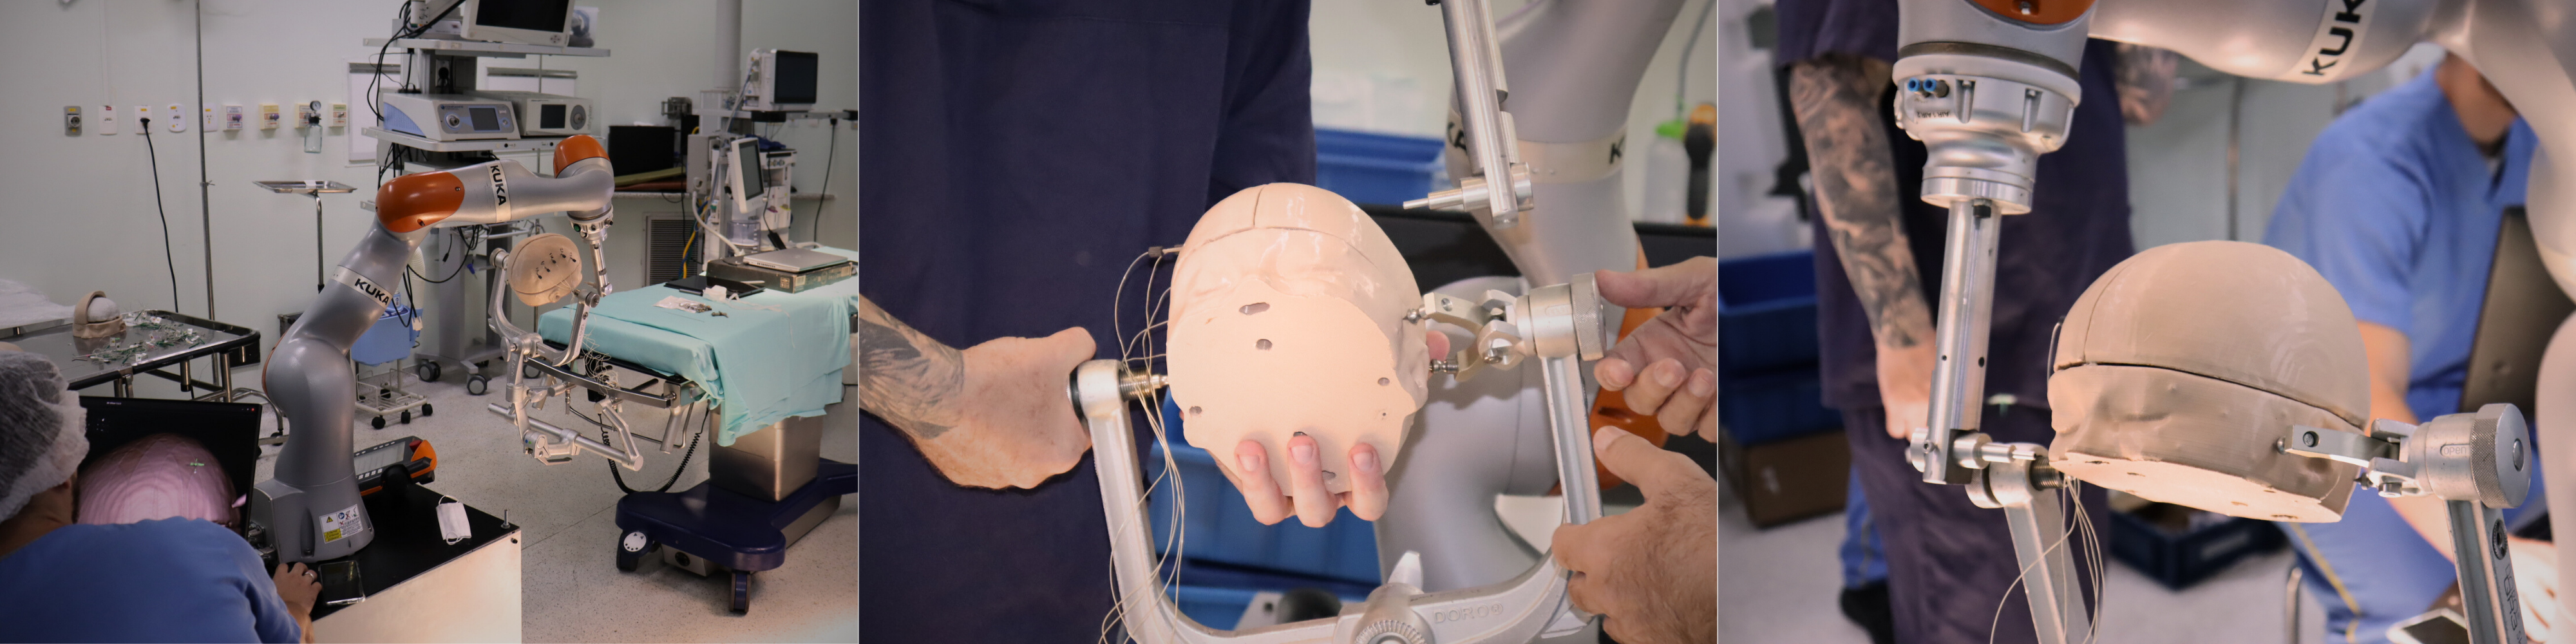
\includegraphics[width=0.95\textwidth]{USPSC-img/synthetic-brain-phantom-or-robot.png}
    \caption{Operating room (OR) with synthetic brain phantom ready for electrode placement using the robotic system.}
    \label{fig:synthetic-or-robot}
\end{figure}

\section{Synthetic Brain Phantom in Operating Room}\label{sec:synthetic-or}

In order to evaluate the system in a real surgical environment, a second synthetic brain model was created. For this phantom, we produced a brain of alginate to better simulate the consistency of real brain tissue. The surface of the head was again 3D printed to replicate the anatomical structure. The phantom was taken to the operating room, where the robotic system was used to perform electrode placement under actual surgical conditions, including the presence of medical staff and adherence to operating room protocols.


\begin{figure}[ht]
    \centering
    \includegraphics[width=0.95\textwidth]{USPSC-img/synthetic-brain-or-ct-leksell.png}
    \caption{Comparison between frame-based planned electrode trajectories (color lines) and those achieved after surgery (showed by the sliced view of the contacts in bright gray) using CT scan of a synthetic brain model in OR with stereotactic frame.}
    \label{fig:synthetic-or-leksell-ct}
\end{figure}

In the right brain hemisphere, we introduced the electrodes using stereotactic frame guidance, while in the left hemisphere, the procedure was performed using the robotic system. This approach allowed for a direct comparison between the traditional frame-based method and the robotic-assisted technique within the same surgical setting. After the procedure, a CT scan was performed to visualize the internal positioning of the electrodes. The postoperative CT images were then fused with the preoperative planning images to assess the accuracy of electrode placement.


\begin{figure}[ht]
    \centering
    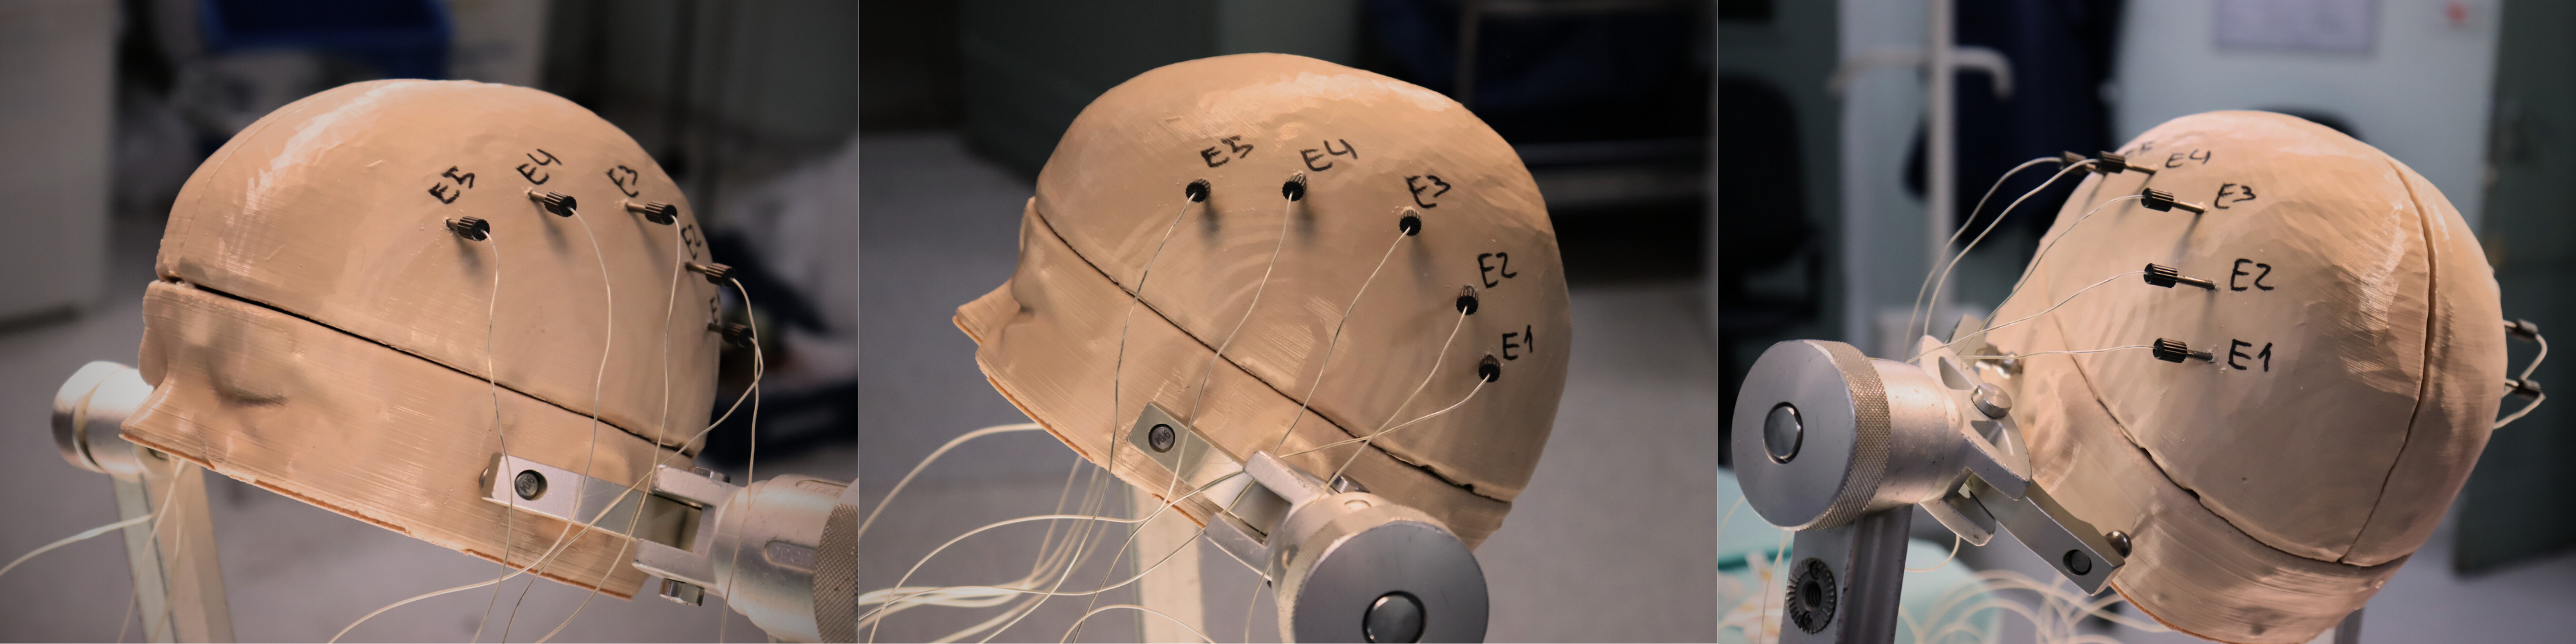
\includegraphics[width=0.95\textwidth]{USPSC-img/synthetic-brain-phantom-or-robot-electrodes.png}
    \caption{Electrodes fixed to the synthetic brain phantom in OR with robotic system.}
    \label{fig:synthetic-electrodes-or-robot}
\end{figure}


\begin{figure}[h]
    \centering
    \includegraphics[width=0.95\textwidth]{USPSC-img/synthetic-brain-or-robot-ct.png}
    \caption{Comparison between planned electrode trajectories (blue lines) and those achieved after surgery (3D contacts in gray) using CT scan of a synthetic brain model in OR with robotic system.}
    \label{fig:synthetic-or-ct-robot}
\end{figure}

For the stereotactic frame procedure, electrode trajectories were planned using preoperative MRI images. In the operating room, the stereotactic frame was securely attached to the phantom's head with the N-Localizer (see Sec. \ref{sec:stereotactics}) and the assembly was transported to the CT scanner for image acquisition. The acquired CT images were fused with the preoperative MRI, enabling precise calculation of electrode coordinates within the frame's coordinate system. Electrode insertion was then performed sequentially, guided by the stereotactic apparatus (Fig. \ref{fig:synthetic-or-leksell}). Finally, a postoperative CT scan was conducted to verify the actual positions of the electrodes (Fig. \ref{fig:synthetic-or-leksell-ct}), fused with the preoperative images, and entry and target errors were calculated (Tab. \ref{tab:synthetic-or-leksell}).


\begin{table}[ht]
    \centering
    \begin{tabular}{|c|ccccc|c|}
        \textbf{Electrode} & \textbf{1} & \textbf{2} & \textbf{3} & \textbf{4} & \textbf{5} & \textbf{Mean} \\
        $\Delta$Entry (mm) & 1.6 & 2.1 & 1.8 & 3.6 & 5.0 & $2.8 \pm 0.25$ \\
        $\Delta$Target (mm) & 8.1 & 16.2 & 11.1 & 15.3 & 13.9 & $12.9 \pm 0.25$ \\
    \end{tabular}
    \caption{Error in positioning the entry and target points planned and reached after surgery using a synthetic brain model in the OR with stereotactic frame.}
    \label{tab:synthetic-or-leksell}
\end{table}

For the robotic procedure, the same preoperative MRI images served as the basis for planning. The phantom was stabilized in the Mayfield head clamp, and anatomical fiducial markers were collected using the robot for registration (Fig. \ref{fig:synthetic-or-robot}). The robot autonomously positioned itself at each planned electrode site, and electrodes were inserted along the preplanned trajectories (Fig. \ref{fig:synthetic-electrodes-or-robot}). Unlike the frame-based approach, no intraoperative CT scan was required, as registration was accomplished directly using the anatomical fiducial markers.


\begin{table}[ht]
    \centering
    \begin{tabular}{|c|cccccc|c|}
        \textbf{Electrode} & \textbf{1} & \textbf{2} & \textbf{3} & \textbf{4} & \textbf{5} & \textbf{Mean} \\
        $\Delta$Entry (mm) & 3.1 & 3.7 & 2.9 & 3.2 & 2.6 & $3.1 \pm 0.25$ \\
        $\Delta$Target (mm) & 5.8 & 5.9 & 5.8 & 5.9 & 5.5 & $5.8 \pm 0.25$ \\
    \end{tabular}
    \caption{Error in positioning the entry and target points planned and reached after surgery using a synthetic brain model in the OR with robotic system.}
    \label{tab:synthetic-or-robot-accuracy}
\end{table}

As in the frame-based procedure, postoperative CT images were fused with preoperative MRI to evaluate electrode placement accuracy. Entry and target errors were calculated by comparing planned and actual electrode positions (Fig. \ref{fig:synthetic-or-ct-robot}, Tab. \ref{tab:synthetic-or-robot-accuracy}).

